
\section{Gradient methods - Part I}

\begin{definition}[smoothness]
	$f : \mathbb{R}^{n}\rightarrow \mathbb{R}$
	is $L$-smooth \textbf{($L$-sm)} if
	$\nabla f(x)$
	satisfies
	$|\nabla f(x)-\nabla f(y)|\le L|x-y|$
	$\forall x,y \in \mathbb{R}^{n}$
\end{definition}

Taylor
$\rightarrow$
$f(y)\le f(x)+\nabla f(x)\T (y-x) +\frac{L}{2}|x-y|^2$

\begin{definition}[strong convexity]
	$f : \mathbb{R}^{n}\rightarrow \mathbb{R}$
	is $\mu$-strongly convex \textbf{($\mu$-scv)} if
	$f(y)\ge f(x)+\nabla f(x)\T(y-x)+\frac{\mu}{2}|x-y|^2$
	% $\forall x,y \in \mathbb{R}^{n}$
\end{definition}

\textbf{How to find $\mu/L$},
Spectra of Hessian $\nabla^2f$, min/max eigenvalue

\subsection{Gradient Descent}

$x_{k+1}=x_k-T\nabla f(x_k)$
for
$k = (k_0,\dots,k_N)$
given
$x_0,T$


Assume
$f(x)=c_0+b\T x+\frac{1}{2}x\T Hx$,
$H\succ0$
$\Rightarrow$
$Hx^\star =-b$

$x_{k+1}-x^\star=x_k-x^\star-T(b+Hx_k)$
$=(I-TH)(x_k-x^\star)$

Convergence given by eigenvalues of $I-TH$,
use $H=U\Lambda U\T$

$x_{N}-x^\star=$
$U(I-T\Lambda)^N U\T(x_0-x^\star)$
$\rightarrow$
conv-rate $1-T\lambda_i$

$f$: $L$-sm, $\mu$-scv
$\rightarrow$
$\mu\le\operatorname{min}\lambda_i$,
$\operatorname{max}\lambda_i\le L$,
$\rightarrow$
conv-rate
$\rho(T)$
$=:\operatorname{max}_{\mu\le h\le L}|1-Th|$
$\rightarrow$
$|x_{N}-x^\star|\le\rho(T)^N|x_{0}-x^\star|$

$T^\star=\frac{2}{L+\mu}$,
with \textbf{condition number}
$\kappa:=\frac{L}{\mu}$
and
$1-\xi\le e^{-\xi}$

$\rho(T^\star)=\frac{L-\mu}{L+\mu}=$
$\frac{\kappa-1}{\kappa+1}=(1-\frac{2}{\kappa+1})$
$\le e^{-\frac{2}{\kappa+1}}$
$\rightarrow$
algebraic complexity
$N\ge\frac{\kappa+1}{2}\operatorname{ln}(\frac{|x_{0}-x^\star|}{\epsilon})$
to achieve
$|x_{N}-x^\star|\le\epsilon$

\subsection{Momentum-based methods}
\vspace{-3.5mm}
\[\begin{aligned}
		q_{k+1} & = q_k + Tp_{k+1}                          \\
		p_{k+1} & = (1-2dT)p_k-T\nabla f(q_k + \beta p_k)/L
	\end{aligned}\]
\vspace{-2.7mm}

\textbf{Nesterov}
accelerated gradient
$T = 1,$
$d=\frac{1}{\sqrt{k}+1}$,
$\beta =\frac{\sqrt{k}-1}{\sqrt{k}+1}$

\textbf{Heavy Ball}
tuned on quadratic
$T = \frac{2\sqrt{k}}{\sqrt{k}+1}$,
$d=\frac{1}{\sqrt{k}+1}$,
$\beta=0$

% 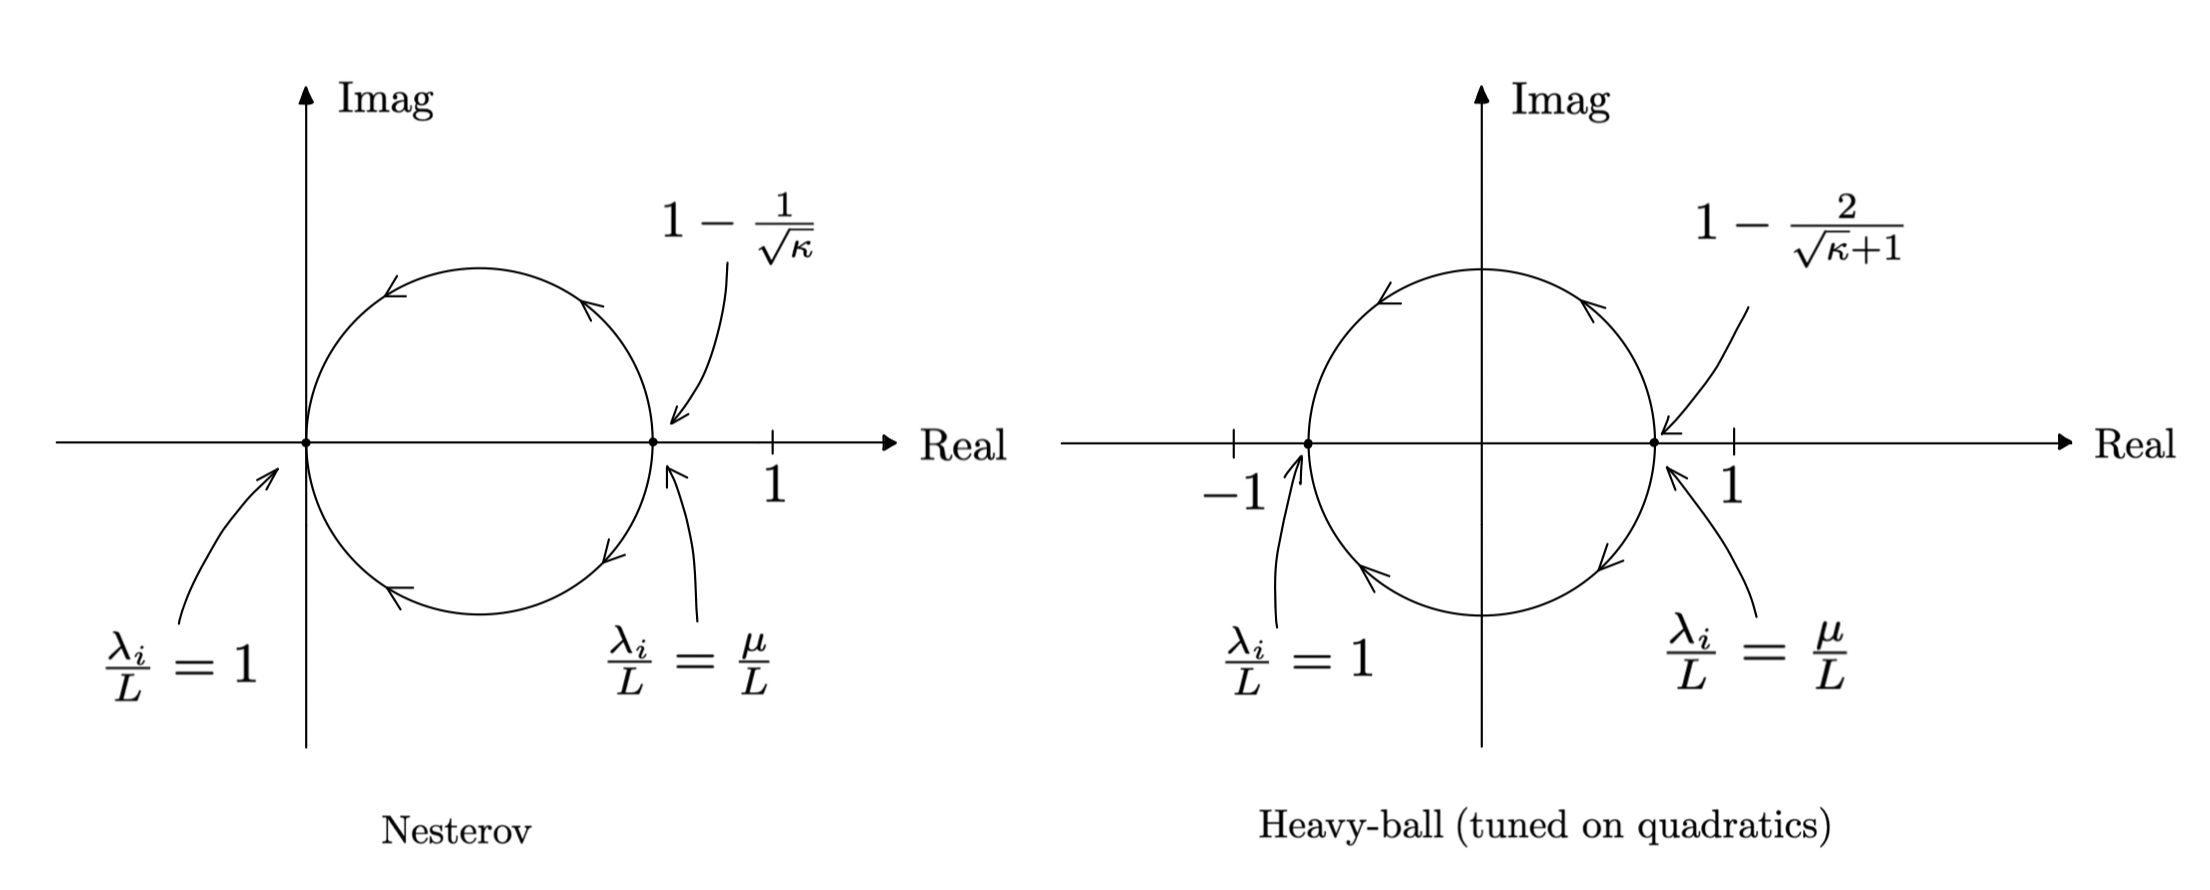
\includegraphics[width=\columnwidth]{images/root-locus-momentum.png}

\begin{centering}
	$C_\text{Nesterov}(1-\frac{1}{\sqrt{\kappa}})^N$
	$\approx\frac{|q_N-q^\star|}{|q_0-q^\star|}\approx$
	$C_\text{HeavyBall}(1-\frac{2}{\sqrt{\kappa+1}})^N$
\end{centering}

\begin{theorem}
	$f$: $L$-sm, $\mu$-scv
	$\rightarrow$
	Nesterov's method satisfies:
	\vspace{-1mm}
	\[  \begin{aligned}
			|q_N-q^\star|  & \le
			\sqrt{\kappa+1}(1-1/\sqrt{\kappa})^{N/2}|q_0-q^\star|
			\\
			f(q_N)-f^\star & \le
			\frac{L+\mu}{2}(1-1/\sqrt{\kappa})^{N}|q_0-q^\star|^2
		\end{aligned}\]
\end{theorem}
\vspace{-1mm}

Requires
$N\ge2\sqrt{\kappa}\operatorname{ln}(\frac{|q_{0}-q^\star|}{\epsilon})$
to achieve
$|x_{N}-x^\star|\le\epsilon$

\begin{theorem}
	For any first-order method
	$\exists f: \mathbb{R}^{\infty}\rightarrow\mathbb{R}$,
	$\mu$-scv, $L$-sm,
	s.t.
	$|x_k - x^\star|\ge$
	$(1-\frac{2}{\sqrt{\kappa}+1})^k|x_0 - x^\star| \forall k\ge 0$

\end{theorem}

\textbf{Line search}
optimal step
$\nu_t^*=\argmin_{\nu\in\mathbb{R}}f(x_t-\nu\nabla f(x_t))$
